\documentclass[11pt]{article}
\usepackage[margin=1in]{geometry}
\usepackage{amsmath,amssymb,amsthm}
\usepackage[hidelinks]{hyperref}
\usepackage{enumitem}
\usepackage{graphicx}

\newtheorem*{remark}{Remark}
\newcommand{\done}{\texttt{done}}

\title{A Better Notation for RL}
\author{Brando Miranda}
\date{November 2026 (draft)}

\begin{document}
\maketitle

\begin{abstract}
A trajectory is written as repeated (reward, state, action) blocks,
$\tau = (r_0, s_0, a_0, \ldots, r_T, s_T, a_T)$. The environment emits each
reward and state together, $P_E(r_t, s_t \mid s_{t-1}, a_{t-1})$, and the agent
emits each action, $P_A(a_t \mid s_t)$. The probability of a trajectory is then
a single product with the same two factors at every step, including the first
and the last. Drawn as a picture, the product separates a rollout (the reward
leaves the loop) from training (the reward changes the weights), which the
usual single agent--environment loop draws together.
\end{abstract}

\section{The trajectory distribution}

Each time step $t$ is one environment draw followed by one agent draw:
\begin{align*}
(r_t, s_t) &\sim P_E(\cdot \mid s_{t-1}, a_{t-1}) && \text{(environment)}\\
a_t &\sim P_A(\cdot \mid s_t) && \text{(agent / policy, usually } \pi_\theta\text{)}
\end{align*}
Written out in full,
\begin{multline*}
P(\tau) = \underbrace{P_E(r_0, s_0 \mid s_{-1}, a_{-1})}_{\text{initial}}\, P_A(a_0 \mid s_0)\;
P_E(r_1, s_1 \mid s_0, a_0)\, P_A(a_1 \mid s_1)\;
P_E(r_2, s_2 \mid s_1, a_1)\, P_A(a_2 \mid s_2) \\
\cdots P_E(r_T, s_T \mid s_{T-1}, a_{T-1})\, \underbrace{P_A(a_T \mid s_T)}_{a_T = \done},
\end{multline*}
which collapses to
\begin{equation}
\boxed{\;P(\tau) = \prod_{t=0}^{T} P_E(r_t, s_t \mid s_{t-1}, a_{t-1})\, P_A(a_t \mid s_t)\;}
\label{eq:traj}
\end{equation}
The return and the value are
\[
R(\tau) = \sum_{t=0}^{T} \gamma^t r_t, \qquad V_E^{P_A} = \mathbb{E}_{\tau \sim P}\big[R(\tau)\big].
\]
This is the indexing of the four-argument dynamics function of Sutton and Barto,
$p(s', r \mid s, a) = \Pr\{S_t = s', R_t = r \mid S_{t-1} = s, A_{t-1} = a\}$,
extended to both ends of the episode.

\section{The first step is not special}

Set $s_{-1} = a_{-1} = \varepsilon$ (empty state and action). Then
\[
P_E(r_0, s_0 \mid s_{-1}, a_{-1}) = P_E(r_0, s_0)
\]
is the initial distribution: the same kernel, with nothing to condition on.
The common convention that the initial state carries no reward is the special
case $r_0 = 0$ almost surely, i.e.
\[
P_E(x, s_0 \mid s_{-1}, a_{-1}) = 0 \quad \text{for all } x \neq 0 .
\]
I prefer not to make the initial step special, since where you start does matter.

\begin{remark}
$r_0$ depends on no action, so it shifts every return by an amount the policy
cannot affect. It changes the value of a start state, not the optimal policy.
\end{remark}

\section{The last step is not special}

The episode ends when the agent acts: $a_T = \done$. The final factor
$P_A(a_T \mid s_T)$ therefore exists, and the product in~\eqref{eq:traj} runs to
$T$ with both factors at every step. For an LLM agent, $a_T$ is the
end-of-sequence token or the tool call that submits an answer.

\section{Two pictures instead of one}

The usual picture of RL is a single loop in which both the next state and the
reward are drawn as inputs to the agent (Figure~\ref{fig:loop}, my redrawing).

\begin{figure}[h]
\centering
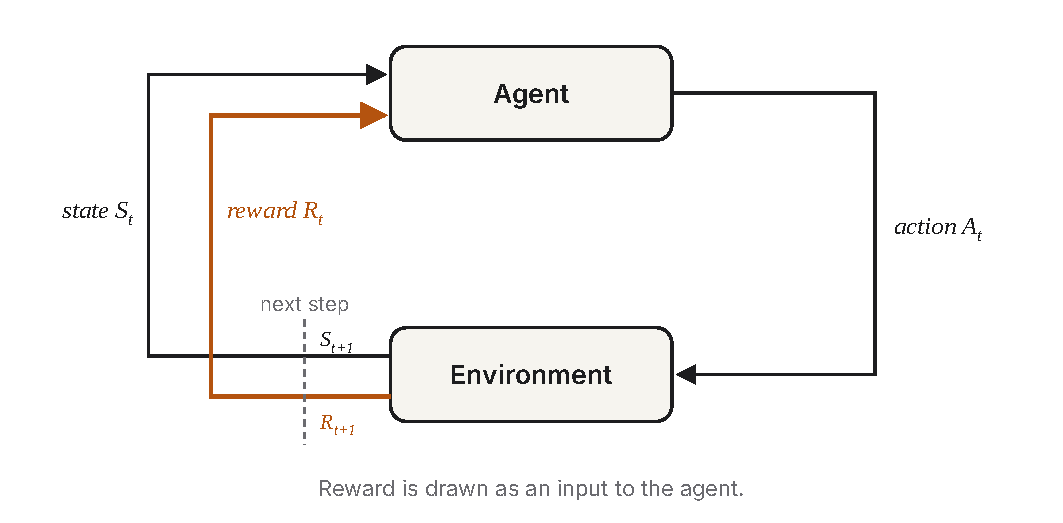
\includegraphics[width=0.72\linewidth]{figs/fig1_textbook_loop.pdf}
\caption{The usual single loop, redrawn. The reward arrow (orange) enters the agent.}
\label{fig:loop}
\end{figure}

During a rollout the policy computes $P_A(a_t \mid s_t)$; no factor takes $r_t$
as an input, so the reward has nowhere to go inside the agent. Drawing only the
arguments of each factor in~\eqref{eq:traj} gives Figure~\ref{fig:rollout}:
$(s_{t-1}, a_{t-1})$ enter the environment, $s_t$ enters the agent, and $r_t$
leaves the loop into the return. The empty start and the $\done$ action appear
explicitly, so both ends are drawn like every other step.

\begin{figure}[h]
\centering
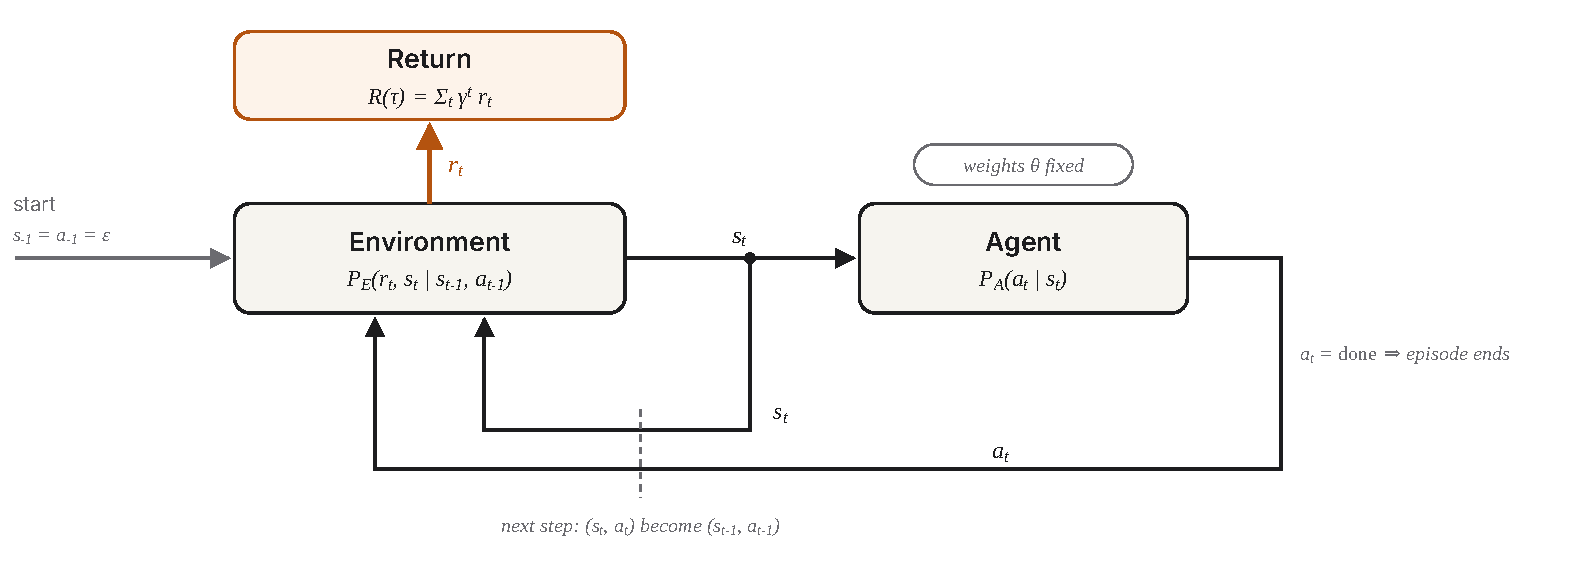
\includegraphics[width=\linewidth]{figs/fig2_rollout.pdf}
\caption{A rollout in this notation. Every arrow is an argument of a factor in
$P(\tau)$. The reward goes to the return, not to the agent; $\theta$ is fixed.}
\label{fig:rollout}
\end{figure}

The reward reaches the agent only during training, and only through the weights:
a learner consumes $r_t$ (and $\log P_A(a_t \mid s_t)$), computes a gradient, and
updates $\theta$ between rollouts (Figure~\ref{fig:train}). The action is still
drawn from $P_A(a_t \mid s_t)$.

\begin{figure}[h]
\centering
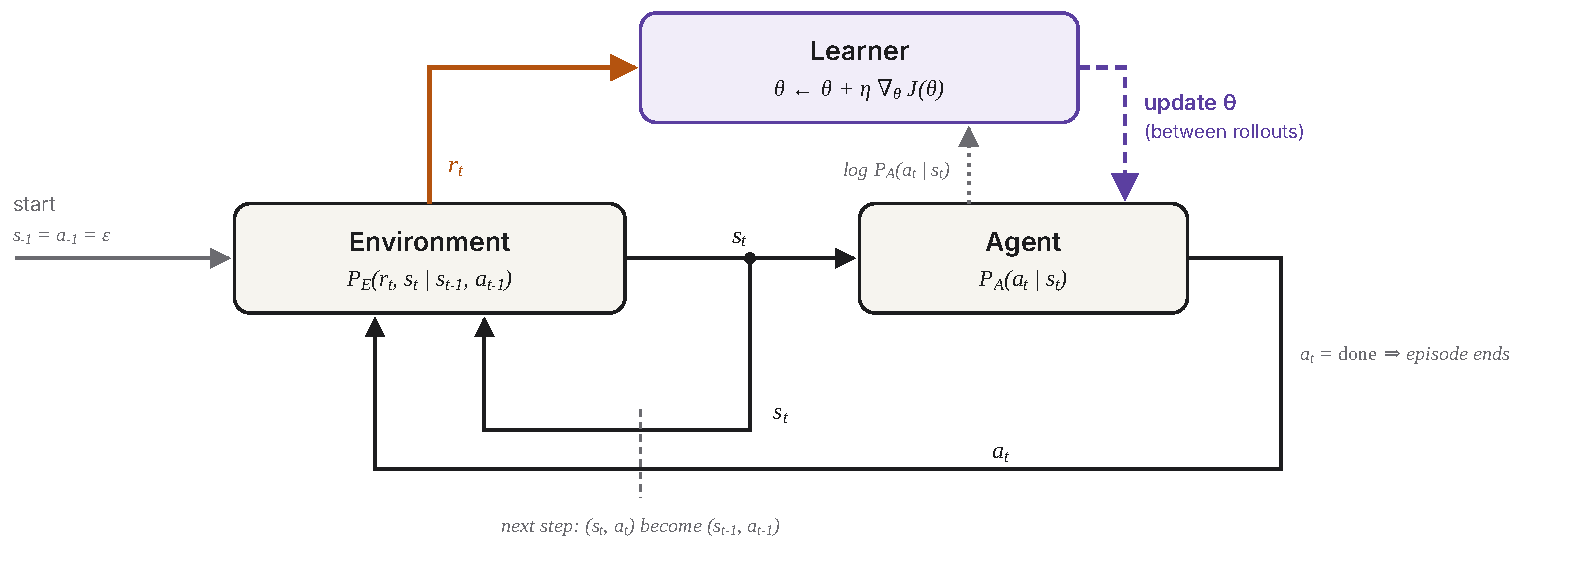
\includegraphics[width=\linewidth]{figs/fig3_training.pdf}
\caption{RL training. The reward is consumed by the learner, which updates $\theta$.}
\label{fig:train}
\end{figure}

\begin{remark}
The single loop draws two systems at once: the policy that acts and the learning
algorithm that changes it. That is a natural choice when the subject is learning
agents. For reading off $P(\tau)$, Figure~\ref{fig:rollout} is the picture of the
distribution and Figure~\ref{fig:train} is the picture of what training does with
it. If a policy is shown rewards (e.g.\ an LLM prompted with the score of its last
attempt), the reward is part of the observation, so it belongs in $s_t$ and the
factor is still $P_A(a_t \mid s_t)$.
\end{remark}

\section{Markov property and time invariance}

Recall conditional independence:
\[
A \perp B \mid C \iff P(A, B \mid C) = P(A \mid C)\, P(B \mid C) \iff P(A \mid B, C) = P(A \mid C).
\]

\paragraph{Markov.} Since $P_E$ conditions only on the previous time step's state
(``location'') and action,
\[
\boxed{\;(r_t, s_t) \perp (r_0, s_0, a_0, \ldots, r_{t-1}) \mid s_{t-1}, a_{t-1}\;}
\]
where the past excludes $s_{t-1}, a_{t-1}$ themselves. Equivalently,
$P(r_t, s_t \mid r_{0:t-1}, s_{0:t-1}, a_{0:t-1}) = P_E(r_t, s_t \mid s_{t-1}, a_{t-1})$:
given $s_{t-1}, a_{t-1}$, anything else on the right-hand side of the bar does not
change the pdf/pmf of $(r_t, s_t)$. Likewise $a_t$ depends on the history only
through $s_t$.

\paragraph{Time invariance.} $P_E$ is the same function at every $t$, including
$t = 0$. This is the symmetry of time in an MDP. Markov and time invariance are
separate properties (a kernel can be Markov and still depend on $t$); a single
$P_E$ inside a single product encodes both.

\begin{remark}[Before, but not after]
The future is not an input to $P_E$: $(r_t, s_t)$ is generated before any later
variable exists. But the future is \emph{not} conditionally independent of
$(r_t, s_t)$, because $s_{t+1} \sim P_E(\cdot \mid s_t, a_t)$, so observing
$s_{t+1}$ is informative about $s_t$. The independence statement is about the
past only; ``the transition doesn't depend on the future'' is a statement about
generation order.
\end{remark}

\end{document}
